\section{Constructing a scaling testbed}
\label{sec:experiments}

\begin{figure}[tp]
    \centering
    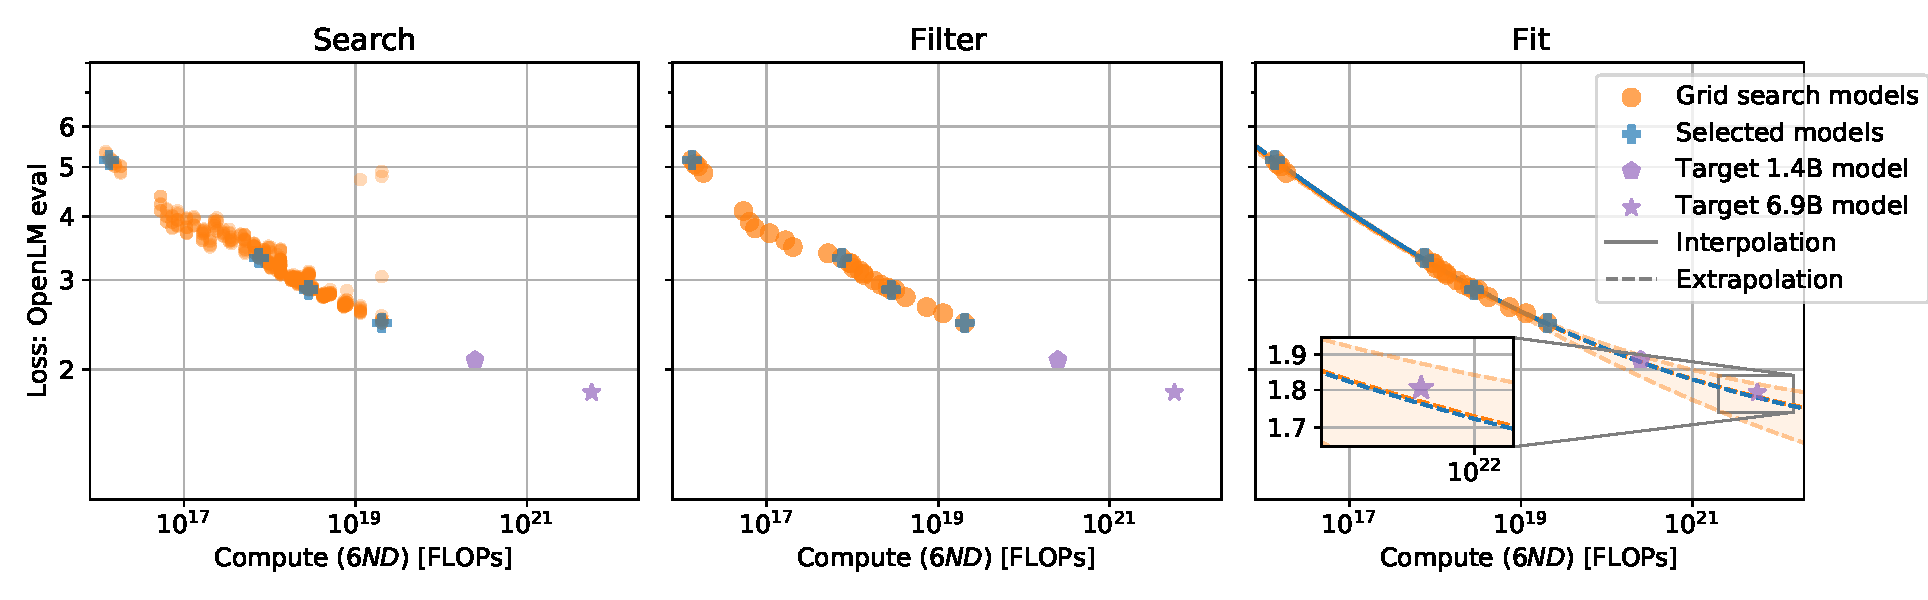
\includegraphics[width=\linewidth]{figs/grid_full.pdf}
    \caption{\textbf{Search, filter, fit:
    A recipe for selecting configurations for scaling.}
    \emph{(left)} To generate the final configurations presented in Table~\ref{tab:hparams}, we run a 435 model grid search over model width, hidden dimension, number of attention heads, batch size, and warmup steps.
    All models are trained near compute-optimally.
    \emph{(center)} We plot the efficient frontier of models, which appear to follow a trend, excluding models from $5.2 \times 10^{16}$ to $5.2 \times 10^{17}$, which fall below the trend.
    \emph{(right)} We fit a power law with irreducible error to the remaining configurations, picking four configurations that closely track the full model suite (``Selected models'').
    These models extrapolate the performance of 1.4B, 6.9B target models.
    Shaded regions represent bootstrap 95\% confidence intervals.
    }
    \label{fig:grid}
\end{figure}

In this section, we discuss our experimental setup to test the predictions suggested by Equations~\eqref{eq:lossCM} and~\eqref{eq:errL}.
We first present our general language modeling setup (Section~\ref{sec:training}).
Next, we discuss our strategy for determining model configurations for our scaling investigation (Section~\ref{sec:searching}) and fitting scaling laws (Section~\ref{sec:fitting}).
We then present metrics to validate how well scaling laws predict loss and downstream performance (Section~\ref{sec:evaluation}).

\subsection{Training setup}
\label{sec:training}

We train transformers~\cite{transformer} for next token prediction, based on architectures like GPT-2~\cite{Radford2019LanguageMA} and LLaMA~\cite{llama}.
We employ GPT-NeoX~\cite{neox} as a standardized tokenizer for all data.
See Appendix~\ref{appx:additional_training_main} for architecture, optimization, and hyperparameter details.

\subsection{Model configurations}
\label{sec:searching}

To get final configurations for the 0.011B to 0.411B parameter models plotted in Figures~\ref{fig:emperical} and~\ref{fig:downstream_corr}, we first conduct a wide grid search over a total of 435 models, trained from scratch, from 0.01B to 0.5B parameters (Figure~\ref{fig:grid}~\emph{(left)}).
We train on the original OpenLM data mix~\cite{open_lm}, which largely consists of RedPajama~\cite{rpj} and The Pile~\cite{pile}.
While we eventually plan to over-train models, at this step we search for \emph{base configurations} near compute-optimality.
We train on 20 tokens per parameter ($M=20$), which, in early experiments, gives models near the compute-optimal frontier.
This is similar to findings in \citet{chinchilla}'s Table 3, which suggests that $M=20$ is near-optimal for the Chinchilla experimental setup.

To find maximally performant small-scale models on validation data, we tune model width, number of layers, number of attention heads, warmup steps, and batch size.
Our validation set, OpenLM eval, contains tokens from recent arXiv papers, the OpenLM codebase itself, and news articles.
We find in early experiments that qk-LayerNorm makes models less sensitive to learning rate, which is a phenomenon \citet{wortsman2023small} report in their Figure 1.
Hence, we fix the learning rate (3$e$-3) for our sweeps.
We also perform smaller grid searches over 1.4B and 6.9B parameter model configurations at $M=20$, retaining the best configurations.

At this point, we have many models, several of which give poor performance; following prior work~\cite{kaplan2020scaling,chinchilla}, we want to keep only models that give best performance.
Hence, in Figure~\ref{fig:grid}~\emph{(center)}, we filter out models that do not lie on the Pareto frontier.
While there appears to be a general trend, configurations between $5.2 \times 10^{16}$ and $5.2 \times 10^{17}$ FLOPs lie below the frontier established by other models.
We hypothesize these models over-perform as they are trained for more optimization steps than their neighbors based on our power-of-two batch sizes.
We provide support for this hypothesis in Appendix~\ref{appx:more_results}, but opt to remove these models from our investigation.

To ensure tractable compute requirements for our scaling experiments, we require a subset of models that follows the trend of the entire Pareto frontier.
In Figure~\ref{fig:grid}~\emph{(right)}, we fit trends to the Pareto models and to a subset of four models.
We notice that the trends closely predict both the performance of the 1.4B and 6.9B models, suggesting that our small-scale configurations reliably extrapolate in the compute-optimal setting.

Moving forward, we do not tune hyperparameters for other token multipliers (i.e., $M \neq 20$), on other training or evaluation distributions, or on validation sets for downstream tasks.
For more details including specific hyperparameters, see Appendix~\ref{appx:additional_training}.

To create our scaling testbed, we start with the four small-scale, base configurations from our grid search: $N\in \{0.011\text{B}, 0.079\text{B}, 0.154\text{B}, 0.411\text{B}\}$.
To ensure our conclusions are not particular to a single training distribution, we train models on each of C4~\cite{c4,c4_ai2}, RedPajama~\cite{rpj}, and RefinedWeb~\cite{refinedweb}, which have 138B, 1.15T, and 600B tokens, respectively, for different token multipliers $M \in \{5, 10, 20, 40, 80, 160, 320, 640\}$.
We omit runs that require more tokens than are present in a dataset (i.e., $N=0.411\text{B}, M=640$ for C4).
We additionally train $N=1.4$B models at $M=20$ and at the largest token multiplier possible without repeating tokens (i.e., 80 for C4, 640 for RedPajama, and 320 for RefinedWeb).
We train $N=6.9\text{B}, M=20$ models on each dataset given the relevance of 7B parameter models~\citep{llama,jiang2023mistral}.
In total this results in a testbed of 104 models.

\subsection{Fitting scaling laws}
\label{sec:fitting}

\begin{table}[tp]
    \centering
    \small
    \caption{\textbf{Default number of parameters $N$ and token multiplier $M$ to fit our scaling laws.}
    We invest $\sim$100 A100 hours to fit Equation~\eqref{eq:lossCM} and $\sim$1,000 A100 hours to fit Equation~\eqref{eq:errL}.} 
    % \vspace*{3mm}
    \begin{tabular}{lccc}
        \toprule
        $N$ & $M$ & Used to fit Equation~\eqref{eq:lossCM} & Used to fit Equation~\eqref{eq:errL} \\\midrule
        0.011B & 20 & \ding{51} & \ding{51}\\
        0.079B & 20 & \ding{51} & \ding{51}\\
        0.154B & 20 & \ding{51} & \ding{51}\\
        0.411B & 20 & \ding{51} & \ding{51}\\
        0.011B & 320 & \ding{51} & \ding{51}\\
        1.4B & 20 & \ding{55} & \ding{51}\\\midrule
        \multicolumn{2}{c}{Total compute $C$ [FLOPs]} & 2.4$e$19 & 2.7$e$20 \\\bottomrule
    \end{tabular}
    
    \label{tab:fit_hparams}
    % \vspace*{-3mm}
\end{table}
We fit Equation~\eqref{eq:lossCM} to approximate $E, a, b, \eta$ using curve-fitting in SciPy~\cite{scipy} (i.e., Levenberg-Marquardt to minimize non-linear least squares).
We repeat this process to fit Equation~\eqref{eq:errL} to approximate $\epsilon, k, \gamma$.
We invest $\sim$100 A100 hours to train the models required to fit a scaling law for loss and $\sim$1,000 A100 hours for a corresponding law for downstream error.
Unless otherwise specified, we fit to the $N, M$ pairs in Table~\ref{tab:fit_hparams}, which are a subset of our full testbed.
Our configurations allow us to test for extrapolation to the $N=1.4\text{B}, M=640$ (900B token) and the $N=6.9\text{B}, M=20$ (138B token) regimes.

\subsection{Evaluation setup}
\label{sec:evaluation}

\paragraph{Evaluation datasets.}
Unless otherwise stated, our default validation loss dataset is C4 eval.
For downstream tasks, we adopt a subset from 46 tasks from LLM-foundry~\cite{mosaicml}, which includes standard tasks with both zero-shot and few-shot evaluations.
Specifically, we consider a 17-task subset where, for each evaluation, at least one 0.154B scale model---trained with as many as 99B tokens---gets 10 percentage points above chance accuracy:
ARC-Easy~\cite{arc},
BIG-bench: CS algorithms~\cite{srivastava2023beyond},
BIG-bench: Dyck languages~\cite{srivastava2023beyond},
BIG-bench: Novel Concepts~\cite{srivastava2023beyond},
BIG-bench: Operators~\cite{srivastava2023beyond},
BIG-bench: QA WikiData~\cite{srivastava2023beyond},
BoolQ~\cite{boolq},
Commonsense QA~\cite{talmor-etal-2019-commonsenseqa},
COPA~\cite{copa},
CoQA~\cite{reddy-etal-2019-coqa},
HellaSwag (zero-shot)~\cite{hellaswag},
HellaSwag (10-shot)~\cite{hellaswag},
LAMBADA~\cite{lambada},
PIQA~\cite{piqa},
PubMed QA Labeled~\cite{pubmed},
SQuAD~\cite{squad},
and
WinoGrand~\cite{winograd}.
For more details on evaluation datasets see Appendix~\ref{appx:eval_data}.
We focus on this subset to ensure we are measuring signal, not noise.
Including downstream tasks like MMLU~\cite{mmlu}, where performance is close to random chance, however, does not invalidate our results as we show in our evaluation set ablations (Appendix~\ref{appx:more_results}).

\paragraph{Metrics.}
We consider three main metrics:
\emph{Validation loss}, which is the cross entropy between a model's output and the one-hot ground truth token, averaged over all tokens in a sequence and over all sequences in a dataset.
\emph{Average top-1 error}, which is a uniform average over the 17 downstream evaluations, as mentioned in the above paragraph.
To measure how good a prediction $\zeta(C, M)$ is, we measure \emph{Relative prediction error}: $|\zeta(C, M) - \zeta_{GT}| / \zeta_{GT}$, where $\zeta$ is the predicted loss $L$ or the average top-1 error $\textsf{Err}$. $\zeta_{GT}$ is the ground truth measurement to predict.

\section{Results: Reliable extrapolation}
\label{sec:results}

In this Section, we quantify the extent to which the scaling laws developed in Section~\ref{sec:method} extrapolate larger model performance using the scaling testbed from Section~\ref{sec:experiments}.
By default, we fit Equations~\eqref{eq:lossCM} and~\eqref{eq:errL} to the configurations in Table~\ref{tab:fit_hparams}, use C4 eval for loss, and the 17-task split from Section~\ref{sec:evaluation} for average top-1 error.
% \vspace*{-2mm}
\begin{figure*}[tp]
    \centering
    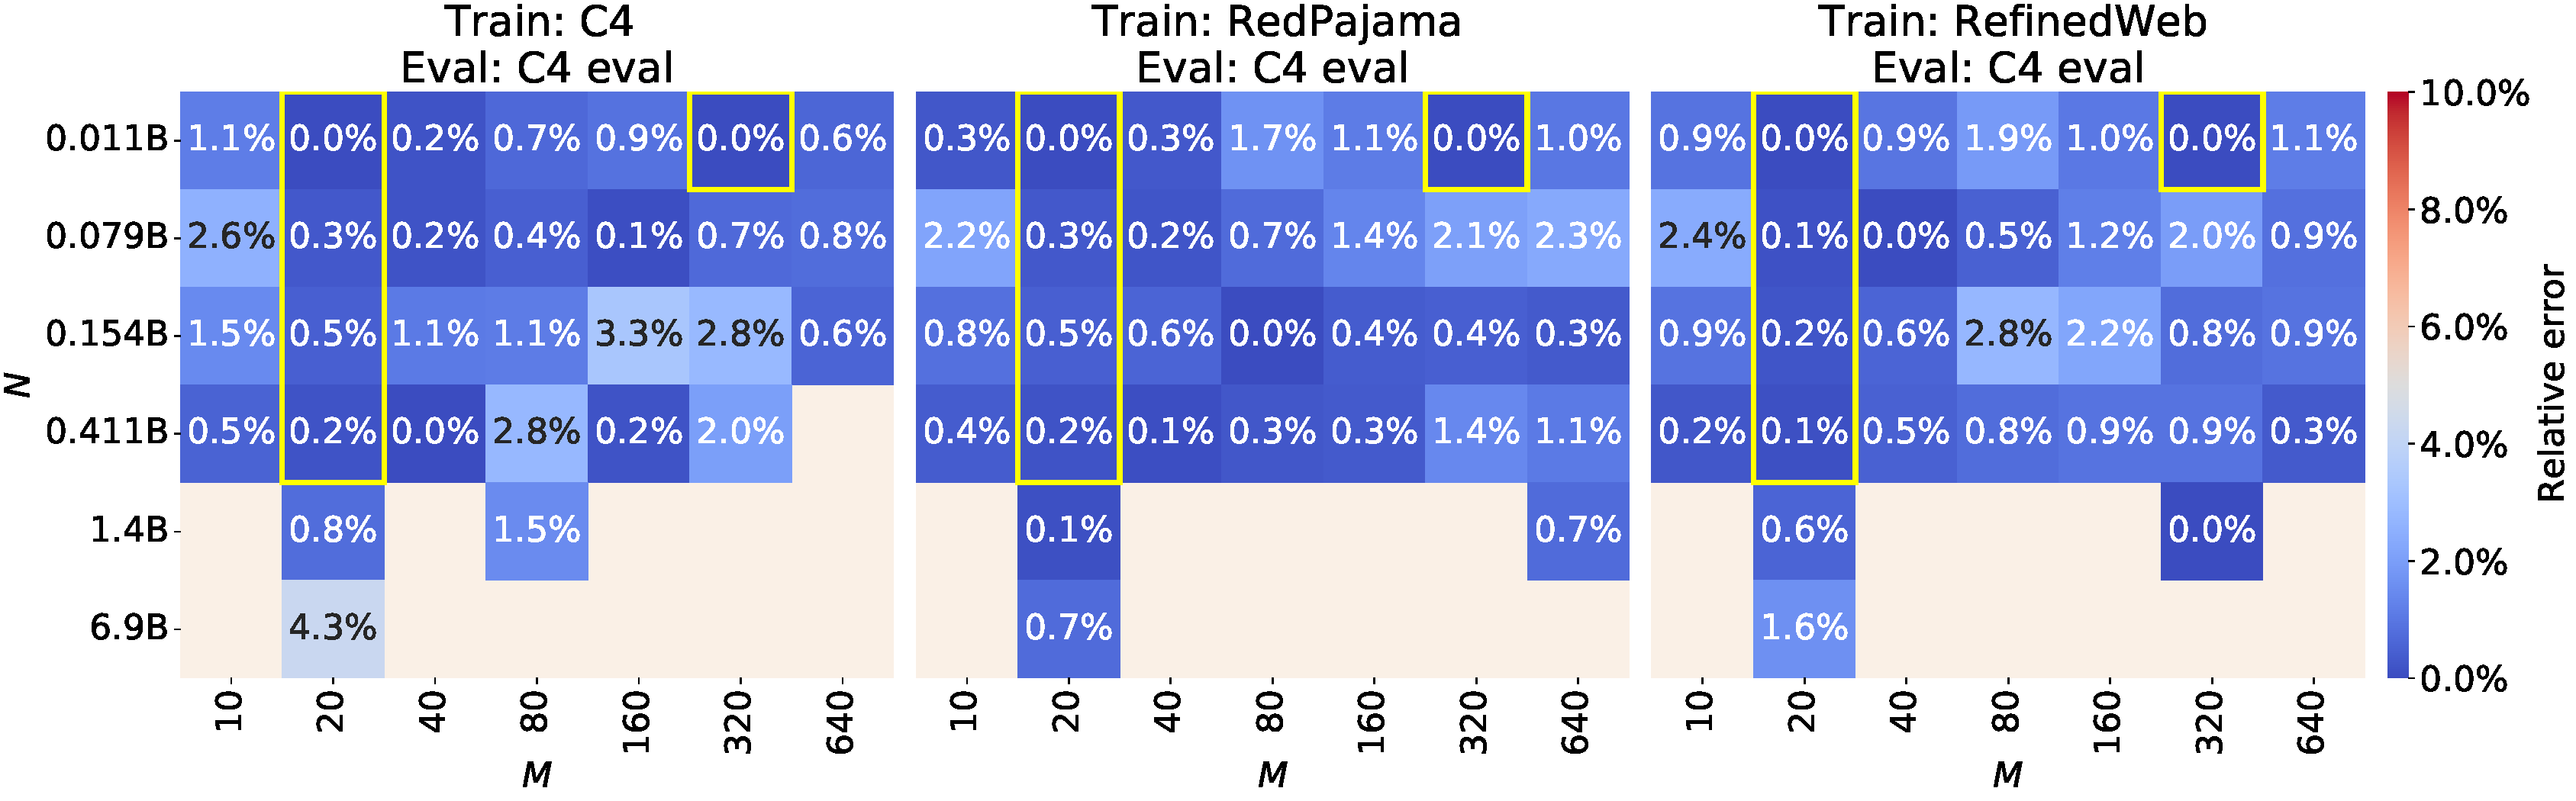
\includegraphics[width=\linewidth]{figs/error.pdf}
    \caption{\textbf{Relative error on C4 eval for different training distributions.} Boxes highlighted in yellow correspond to pairs---number of parameters $N$, token multiplier $M$---used to fit Equation~\eqref{eq:lossCM}. Larger values of $M$ correspond to more over-training. The prediction error is low in both interpolation and extrapolation ranges. Below $N=1.4$B, empty squares correspond to runs that were not possible due to the limited dataset size for single epoch training. At $N=1.4$B we run at $M=20$ and at the largest possible multiplier. At $N=6.9$B, we run at $M=20$.}
    \label{fig:error}
    % \vspace*{-2mm}
\end{figure*}

\paragraph{Over-trained performance is predictable.}
We highlight our main over-training results in Figure~\ref{fig:fig1}~\emph{(left)}.
Namely, we are able to extrapolate both in the number of parameters $N$ and the token multiplier $M$ to closely predict the C4 eval performance of a 1.4B parameter model trained on 900B RedPajama tokens ($N=1.4\text{B}, M=640$).
Our prediction, which takes 300$\times$ less compute to construct than the final 1.4B run, is accurate to within 0.7\% relative error.
Additionally, for the $N=6.9\text{B}, M=20$ run, near compute-optimal, the relative error is also 0.7\%.

These results support several key takeaways.
(i) Scaling can be predictable even when one increases both the model size and the amount of over-training compared to the training runs used to fit a scaling law.
(ii) The form presented in Equation~\eqref{eq:lossCM} is useful in practice for predicting over-trained scaling behavior.
(iii) Fitting to Equation~\eqref{eq:lossCM} gives good prediction accuracy near compute-optimal.
More specifically, predictions are accurate both for the 1.4B over-trained model and the 6.7B compute-optimal model using a single scaling fit.

While Figure~\ref{fig:fig1} explores a specific case of making predictions in the over-trained regime, we aim to understand the error profile of our predictions across training datasets, token multipliers, and number of parameters.
Hence, Figure~\ref{fig:error} shows the relative error between ground truth loss and predicted loss on C4 eval for models in our testbed.
We notice uniformly low prediction error suggesting that predictions are accurate in many settings.

% \vspace*{-2mm}
\paragraph{Average top-1 error is predictable.}
Figure~\ref{fig:fig1}~\emph{(right)} presents our main result in estimating scaling laws for downstream error.
Concretely, we use the models indicated in Table~\ref{tab:fit_hparams} to fit Equations~\eqref{eq:lossCM} and~\eqref{eq:errL}, chaining the scaling fits to predict the average top-1 error as a function of training compute $C$ and the token multiplier $M$.
Our fits allow us to predict, using $20\times$ less compute, the downstream performance of a 6.9B model trained on 138B RedPajama tokens to within $0.05\%$ relative error and a 1.4B model trained on RedPajama 900B tokens to within $3.6\%$ relative error.

Table~\ref{tab:downstream} additionally shows the relative error of our downstream performance predictions for models trained on C4, RedPajama, and RefinedWeb, indicating that our scaling law functional forms are applicable on many training datasets.
We note that while average accuracy is predictable, \textit{individual} downstream task predictions are significantly more noisy.
We report relative error for more model predictions in Figures~\ref{fig:error_downstream_all} and \ref{fig:error_downstream_subset}.
We also find that if we remove the 1.4B model for the Equation~\eqref{eq:errL} fit, relative error jumps, for instance, from 0.05\% to 10.64\% on the 17-task split for the 6.9B, 138B token RedPajama prediction.
This highlights the importance of investing more compute when constructing scaling laws for downstream task prediction compared to loss prediction.

\begin{table}[tp]
    \centering
    \caption{
    \textbf{Downstream relative prediction error at 6.9B parameters and 138B tokens.}
    While predicting accuracy on individual zero-shot downstream evaluations can be challenging (``Individual''), predicting \textit{averages} across downstream datasets is accurate (``Avg.'').
    }    
    \resizebox{\linewidth}{!}{
    \begin{tabular}{lcccc@{\hskip 8ex}c}
        \toprule
        & \multicolumn{4}{c}{Individual top-1 error} & {Avg. top-1 error} \\
        \cmidrule(lr){2-5} \cmidrule(lr){6-6}
         Train set & ARC-E~\cite{arc} & LAMBADA~\cite{lambada} & OpenBook QA~\cite{OpenBookQA2018} & HellaSwag~\cite{hellaswag} & 17-task split \\\midrule
         C4~\cite{c4,c4_ai2} & 28.96\% & 15.01\% & 16.80\% & 79.58\% & 0.14\% \\
         RedPajama~\cite{rpj} & 5.21\% & 14.39\% & 8.44\% & 25.73\% & 0.05\% \\
         RefinedWeb~\cite{refinedweb} & 26.06\% & 16.55\% & 1.92\% & 81.96\% & 2.94\% \\ 
        \bottomrule
    \end{tabular}
    }
    % \vspace*{2mm}
    \label{tab:downstream}
    % \vspace*{-6mm}
\end{table}

% \vspace*{-3mm}
\paragraph{Under-training, out-of-distribution scaling, compute-reliability trade-offs.}
In addition to our main results presented above, we include additional results in Appendix~\ref{appx:more_results}, which we summarize here.
First, we notice that when token multipliers become too small (i.e., $M=5$) scaling becomes unreliable and lies off the trend.
Additionally, multipliers other than 20, such as 10, 40, and 80, garner points that are roughly on the compute optimal frontier (Figure~\ref{fig:emperical_small}).
This observation suggests that the compute-optimal multiplier may lie in a range rather than take a single value.
To probe the limits of reliable scaling, we attempt to break our scaling laws in out-of-distribution settings.
We find that models trained on C4---English filtered---and evaluated on next token prediction on code domains have a high relative error in many cases. Perhaps surprisingly, evaluating the same models on German next token prediction gives reliable loss scaling (Figure~\ref{fig:error_ood}).
We additionally examine the compute necessary to create accurate scaling laws, finding
that scaling laws can be constructed more cheaply for loss prediction than for downstream error prediction (Figures~\ref{fig:error_vs_1b} and~\ref{fig:error_vs_7b}).

